\section{Implementierung von Event Sourcing}
\label{sec:implementation:eventSouring}
Wie bereits erwähnt basiert die persistenz der Daten auf dem im Abschnitt \ref{sec:eventSourcing} beschriebenen \textit{Event Sourcing}. Das Prinzip von \textit{Event Sourcing} ist es, aufgetretene Ereignisse abzuspeichern und gegebenenfalls wieder einzuspielen um so einen Zustand reproduzieren und nachvollziehen zu können. \\
Das verwendete Framework \textit{Akka.net} bietet Grundsätzliche Unterstützung für \textit{Event Sourcing}. Dabei werden Events als Nachrichten repräsentiert, welche dem Framework übergeben werden und anschließend abgespeichert werden. Nach erfolgreicher Speicherung des Events kann auf das aufgetretene Event reagiert werden. Weiters bietet \textit{Akka.Net} die Möglichkeit Events wieder einzuspielen und mit einer gesonderten Reaktion darauf zu reagieren. Dies ist erforderlich damit Ereignisse welche in der Vergangenheit aufgetreten sind, zwar wieder eingespielt werden können, jedoch wird die Einspielung meist anders behandelt als wie wenn das Ereignisse gerade aufgetreten ist. Beispielsweise wird bei einem Ticketbuchung das Bankkonto belastet, wird die Buchung nachträglich wieder eingespielt sollte zwar der Status des Tickets aktualisiert werden, eine neuerliche Kontobelastung ist aber nicht erforderlich. 

\subsection{Aggregate Root}
Um die Implementierung der einzelnen Entitäten zu vereinfachen, wurde die Logik für \textit{Event Sourcing} in einer basis Klasse zusammengeführt, von welcher die eigentlichen Entitäts Actoren ableiten. 
Die basis Klasse bietet die Methode \textit{Emit(IDomainEvent e, Action a)} an, welche die eigentliche Logik für die Speicherung des Events übernimmt. Der Verwender der Methode \textit{Emit()} übergibt dieser ein Event, welche alle Informationen über das aufgetretene Ereignis enthält. Weiters wird eine Action übergeben, welche ausgeführt wird, sobald das Event erfolgreich im \textit{Event Store} abgelegt wurde. Während der Speicherung des Events wird von \textit{Akka.net} sichergestellt, dass keine weitere Nachrichten vom Actor abgearbeitet werden. Die Methode \textit{Emit()} speichert jedoch nicht nur das Event im \textit{Event Store} ab. Bevor es nach der Speicherung des Events die übergebene Action ausführt, wird die abstrakte Methode \textit{UpdateState()} aufgerufen. \\
Jede Ausprägung der abstrakten \textit{Aggregate Root} Klasse muss die Methode \textit{UpdateState(IDomainEvent e)} implementieren. Diese wird wie bereits erwähnt direkt nach der erfolgreichen Persistierung des Events von der Methode \textit{Emit()} aufgerufen. Die Implementierung der Methode \textit{UpdateState()} sollte den Zustand des repräsentierten Actors entsprechend dem aufgetretenen Event verändern. Im Gegensatz zu der zuvor übergebenen \textit{Action}, wird \textit{UpdateState()} auch bei einer historischen Einspielung der Events aufgerufen. Die Methode \textit{UpdateState()} sollte mit jedem allen unterschiedlichen Event Varianten umgehen können und dementsprechend die interne Repräsentation des Actors verändern. Das führt dazu, dass änderungen der Repräsentation des Actors, ausserhalb der Methode \textit{UpdateState()}, bei einer wiedereinspielung der Ereignisse zu unterschiedlichen Zuständen des Actors führen können. Deshalb sollten sämtliche änderungen des Zustandes innerhalb der Methode \textit{UpdateState()} ausgeführt werden. \\
Nach dem aktualisieren des Actors State prüft die Methode ob ein \textit{Snapshot} ausführt werden soll, siehe dazu den folgenden Abschnitt \ref{subsec:implementation:eventSouring:Snapshot}. Abschließend wird die übergebene Methode \textit{Action} aufgerufen, welche die Logik enthält wie auf das aufgetretene Ereignis reagiert wird. Unter anderem können hier andere Actors über das aufgetretene Ereignis benachrichtigt werden. \\
In der Abbildung \ref{fig:implementation:eventSourcingAggregateRoot} ist der beschriebene Prozess schematisch abgebildet. Daraus ist auch zu entnehmen das zwei unterschiedliche Datenbanken verwendet werden um den Snapshots und Events zu speichern.
\begin{figure}
    \centering
    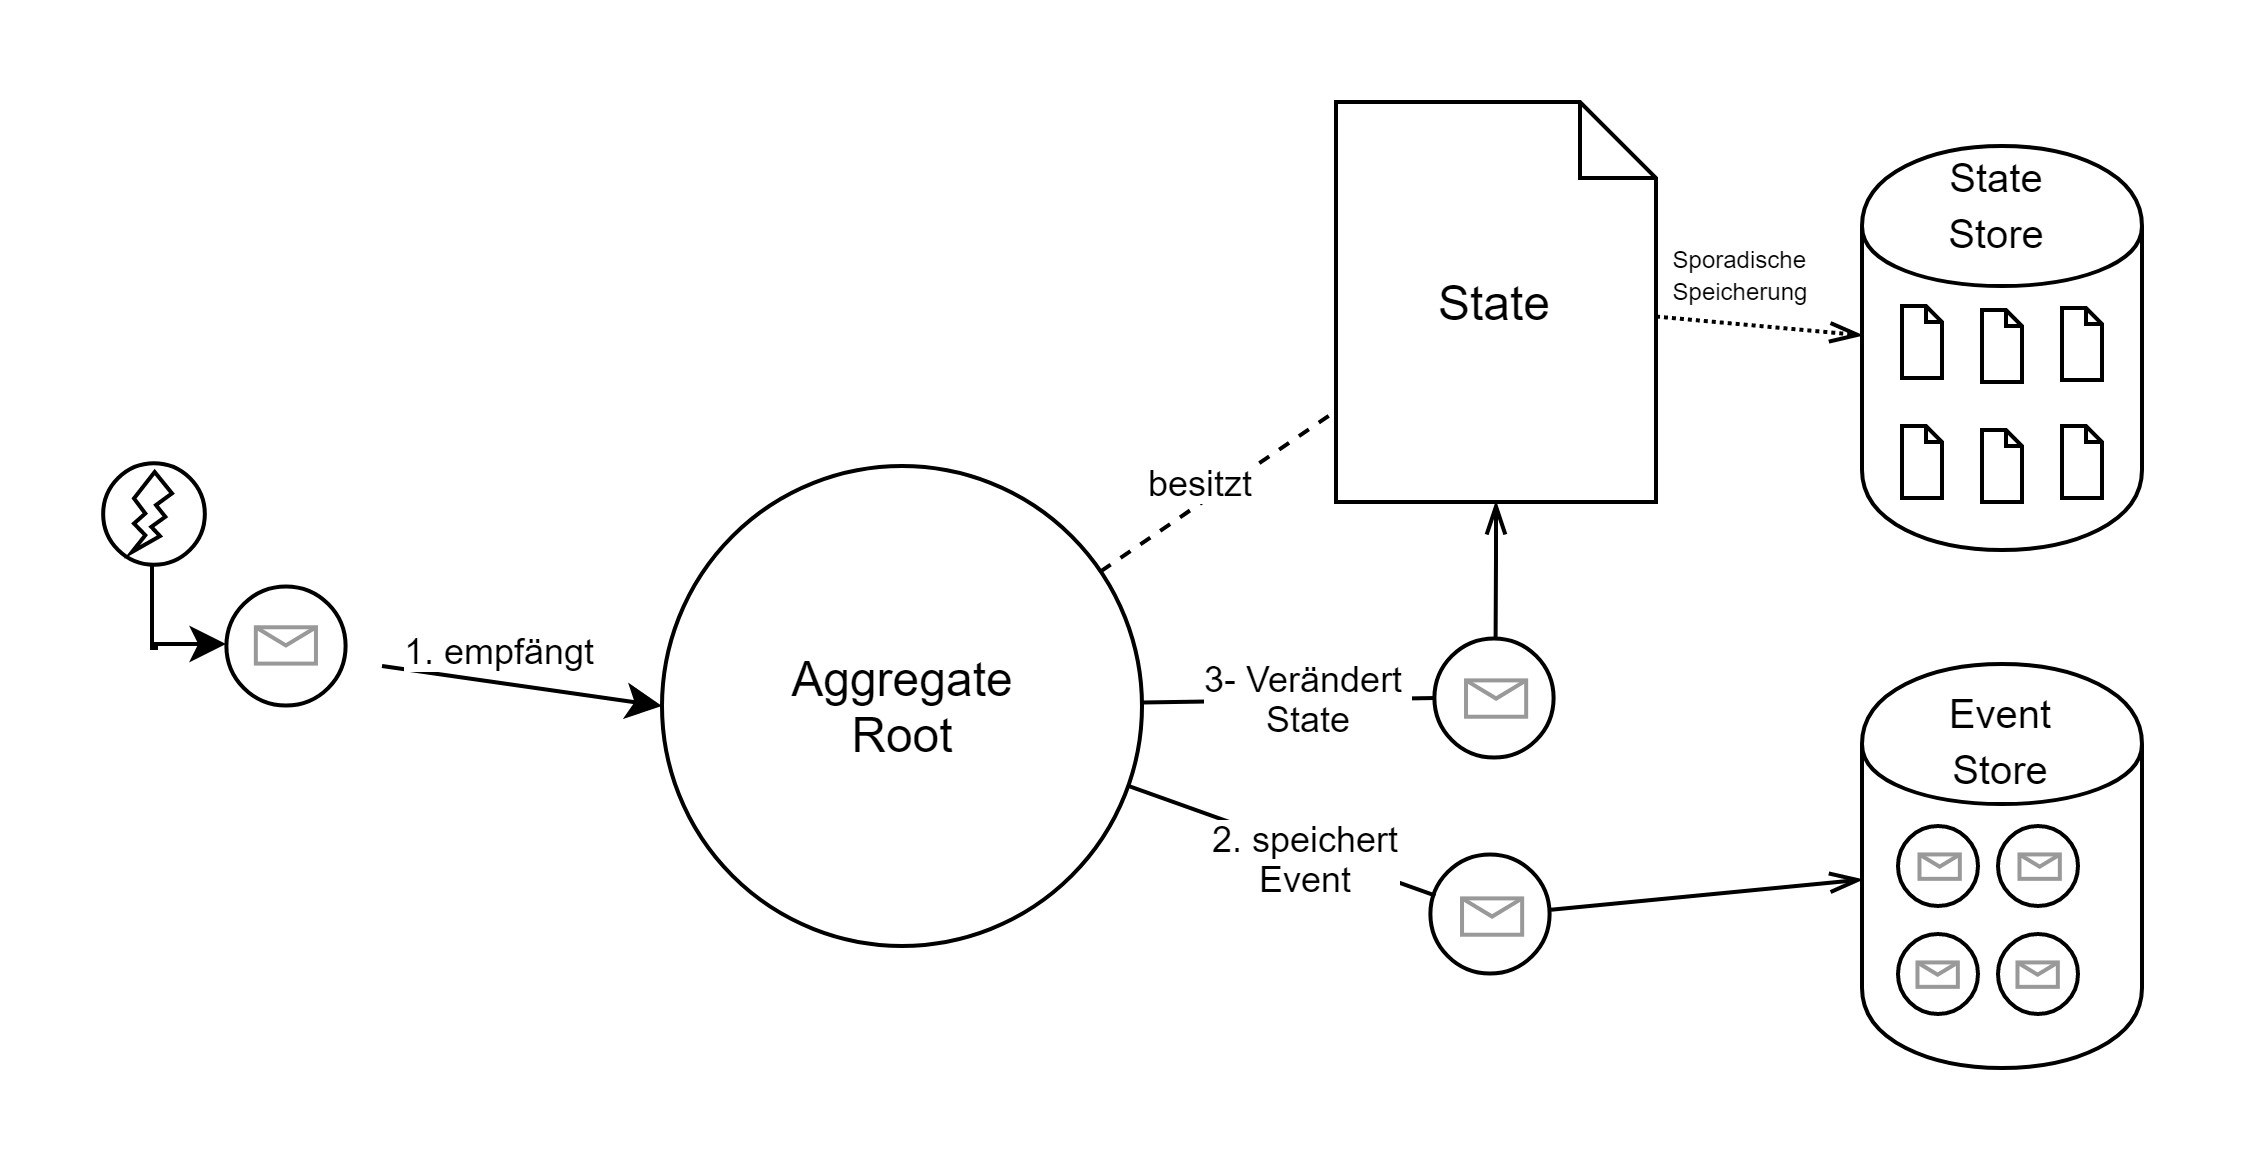
\includegraphics[width=\linewidth]{gfx/implementation/EventSourcingAkka}
    \caption{Ablauf der Speicherung eines Events innerhalb eines \textit{Aggregate Root} Actors mit \textit{Event Sourcing} und \textit{Snapshots}.}
    \label{fig:implementation:eventSourcingAggregateRoot}
\end{figure} 

\subsection{Snapshot}
\label{subsec:implementation:eventSouring:Snapshot}
Um bei einer Wiedereinspielung der Ereignisse für einen Actor nicht alle vergangenen Ereignisse einspielen zu müssen, und dabei für jedes Ereignis die Methode \textit{UpdateState()} aufrufen zu müssen, wird regelmäßig ein Abbild des aktuellen Zustand gespeichert. Dies passiert innerhalb der Methode \textit{Emit()}. In der vorliegenden Implementierung wird nach jedem zwanzigsten Event ein Snapshot erstellt. Dafür wird die interne Datenrepräsentation eines Actors in eine eigene serialisierbare Klasse, den \textit{Actor State}, abgebildet. Diese Klasse wird auch bei der oben besprochenen Methode \textit{UpdateState()} verändert. Wird nun ein Snapshot erstellt, so wird der aktuelle \textit{Actor State} in einer dafür vorgesehenen Datenbank abgespeichert. Zusätzlich zum aktuellen \textit{State} wird die Sequence Nummer des letzten Events, welches zu diesem \textit{State} geführt, hat gespeichert. Während der Erstellung des Snapshots, kann der Actor selbst jedoch weiterhin Nachrichten abarbeiten. Dies beinträchtigt nicht die konsistenz der Datenrepräsentation. Durch die Zuordnung von Sequence Nummer zu einem \textit{State} werden Events welche während der erstellung des Snapshots anfallen, nicht mehr zum Snapshot gezählt und werden später wieder auf Basis des vorhandenen Snapshots eingespielt. \\
Wird nun ein gestoppter Actor, dessen Zustand mittels \textit{Event Sourcing} persistiert wurde, wieder gestartet, so wird bevor er Nachrichten abarbeiten kann der  vorherige Zustand wieder hergestellt. Dies passiert, in dem zuerst der zuletzt verfügbare \textit{Snapshot} gesucht und anschließend dem Actor zugewiesen wird. Nun werden alle Events welche nach der erstellung dieses Snapshots angefallen sind, in der Reihenfolge deren auftretten, wieder in den Actor eingespielt. Nach dem letzten Event, ist der Zustand exakt der gleiche wie vor dem Stoppen des Actors.

\subsubsection{Actors mit \textit{Event Sourcing}}
Wie bereits angedeutet sind nicht alle Actors innerhalb der \textit{TyrolSky} Anwendung unter \textit{Event Sourcing}. Nur Actors welche einen Zustand repräsentieren welche für die konsistenz der Anwendung notwending ist, wurden mit \textit{Event Sourcing} persistiert. Dies sind folgende Actors: 
\begin{itemize}
    \item{\textit{OperateFlight}}
    \item{\textit{FlightPassangerList}}
    \item{\textit{ChargingCoordinator}}
    \item{\textit{FlightTicket}}
    \item{\textit{FlightNumber}}
    \item{\textit{DistributedUniqueNamingService}}
\end{itemize}
Alle bis auf den Actor \textit{DistributedUniqueNamingService} sind Teile der Komponente \textit{Domain Service} und Präsentieren die Domäne der \textit{TyrolSky}. Der verbleibende Actor \textit{DistributedUniqueNamingService} dient zur Implementierung der unterschiedlichen \textit{Query} Aufbereiter der \textit{Query-Service} welche bereits in Abschnitt \ref{subsubsub:implementation:queryActorModel:resultPreparator} beschrieben wurden.

\subsection{Version Problematik}
Durch die Möglichkeit bereits aufgetretene Events immer wieder dem Actor einzuspielen, muss sichergestellt werden, dass Events bei einer Wiedereinspielung gleich behandelt werden, wie zu dem Zeitpunk, als das Ereignis tatsächlich aufgetreten ist. Ändert sich die Implementierung für einen bestimmten Event-Typ innerhalb der Methode \textit{UpdateState()}, welche wie besprochen auch vergangene Events verarbeitet. So muss entschieden werden, ob diese Änderung auch für ältere Events zulässig ist. Denn wird durch die Codeanpassung nun für Events ein anderer Actor State berechnet, kann nicht mehr der Originalzustand zum Zeitpunk des Ereignisses herbeigeführt werden. \\
Deshalb wird, sollte ein neues Verhalten für ein Event benötigt werden, ein neuer Event-Typ eingeführt. Durch die Versionierung von Event-Typen können keine inkonsistenzen durch Codeänderungen in das System gebracht werden. 

